\documentclass[border=2pt]{standalone}
\usepackage{tikz}

\begin{document}
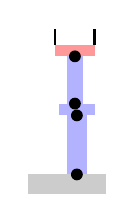
\begin{tikzpicture}[scale=0.5]
    % Robot base
    \fill[gray!40] (0,0) rectangle (2,0.5);

    % Robot arm segments
    \fill[blue!30] (1,0.5) rectangle (1.5,2);
    \fill[blue!30] (0.8,2) rectangle (1.7,2.3);
    \fill[blue!30] (1,2.3) rectangle (1.4,3.5);

    % End effector
    \fill[red!40] (0.7,3.5) rectangle (1.7,3.8);
    \draw[thick] (0.7,3.8) -- (0.7,4.2);
    \draw[thick] (1.7,3.8) -- (1.7,4.2);

    % Joints
    \fill[black] (1.25,0.5) circle (0.15);
    \fill[black] (1.25,2) circle (0.15);
    \fill[black] (1.2,2.3) circle (0.15);
    \fill[black] (1.2,3.5) circle (0.15);
\end{tikzpicture}
\end{document}
